\documentclass{../note}

\begin{document}

\begin{zadanie}{322}
Niech $\mathbb{Z}[x]$ oznacza zbiór wszystkich wielomianów zmiennej $x$ o współczynnikach całkowitych i niech $r$ będzie taką relacją w zbiorze $\mathbb{Z}[x]$, że $\langle f,g\rangle\in r$ zachodzi wtedy i tylko wtedy, gdy różnica $f-g$ ma wszystkie współczynniki parzyste.
\begin{enumerate}
    \item[(a)] Pokazać, że $r$ jest relacją równoważności.
    \item[(b)] Wskazać trzy różne klasy abstrakcji.
    \item[(c)] Jakiej mocy jest zbiór wszystkich klas abstrakcji?
    \item[(d)] Wskazać wszystkie liczby kardynalne, które są mocami klas abstrakcji tej relacji.
\end{enumerate}
\end{zadanie}
\begin{rozwiazanie}
\begin{enumerate}[label=(\alph*)]
    \item $r$ jest zwrotne, bo dla dowolnego wielomianu $f \in \Z[x]$ zachodzi $f - f = 0$, a wielomian zerowy ma współczynniki zerowe, czyli parzyste. Jeśli współczynnik wielomianu $f - g$ przy $x^n$ to $a_n$, to współczynnik $g - f$ przy $x^n$ to $-a_n$. Zachodzi $a_n \equiv -a_n \mod 2$ dla dowolnego $a_n \in \Z$, więc $r$ jest symetrzyczne. Jeśli $\langle f,g\rangle, \langle g,h\rangle\in r\in r$ i współczynniki $f, g, h$ przy $x^n$ to odpowiednio $f_n, g_n, h_n$, to $f_n \equiv g_n \equiv h_n \mod 2$, czyli $f_n \equiv h_n \mod 2$. To zachodzi dla każdego $n$, zatem $r$ jest przechodnia. Zatem $r$ jest relacją równoważności.
    \item Wszytkie wielomiany z parzystymi współczynnikami, wszystkie wielomiany z niepa\-rzystymi współczynnikami i wszystkie wielomiany, w których parzystość współczynników jest taka sama, jak parzystość potęgi, przy której jest dany współczynnik. Łatwo sprawdzić, że te klasy są parami rozłączne, bo mają różne wspóczynniki przy $x^0$ lub $x^1$, że wszystkie trzy są pełne (tzn. nie można dołożyć wielomianów do żadnego z nich), bo np. jeśli jakiś współczynnik jakiegoś wielomianu nie jest parzysty, to nie jest w relacji z wielomiamianami, które mają wszystkie współczynniki parzyste, oraz że w każdej z tych trzech klas, każda para wielomianów jest w relacji.
    \item Zauważmy, że warunek "$f-g$ ma wszystkie współczynniki parzyste" jest równoważny warunkowi "$f$ i $g$ mają wspóczynniki o takiej samej parzystości przy tych samych potęgach". Mamy więc bijekcję pomiędzy $\N/_r$ a $\{0, 1\}^\N$, bo każdej klasie abstrakcji możemy przypisać takie $h \in \{0, 1\}^\N$, że $h(n) = 1$ wtedy i tylko wtedy, gdy wielomiany w tej klasie mają nieparzysty współczynnik przy $x^n$. Mamy więc $|\N/_r| = |{0, 1}^\N| = \mathfrak{c}$.
    \item Niech $A \in \N/_r$. Wiadomo, że $A \subseteq \Z[x]$, czyli $|A| \leq |\N^\N|$. Niech $h \in \{0, 1\}^\N$ to funkcja, którą przypisaliśmy $A$ w poprzednim podpunkcie. Możemy skonstruować funkcję $\phi : \N^\N \to A$ w taki sposób, że gdy $f \in \N^\N$, to $a_{\phi(f)(n)} = 2f(n) + h(n)$. $\phi$ jest dobrze zdefiniowana, bo $2f(n) + h(n) \equiv h(n) \mod2$. $\phi$ jest różnowartościowa, bo jeśli $f, g \in \N^\N$ są różne, to $2f(n) + h(n) \neq 2g(n) + h(n)$ dla pewnego $n$. Zatem $|A| = |\N^\N| = \mathfrak{c}$ dla każdego $A \in \N/_r$.
\end{enumerate}
\end{rozwiazanie}

\begin{zadanie}{349}
Niech $\mathcal{R}$ będzie zbiorem wszystkich relacji równoważności w zbiorze $\mathbb{N}$ i niech $g:\mathcal{R}\rightarrow \mathsf{P}(\mathsf{P}(\mathbb{N}))$ będzie taka, że $g(r)=\mathbb{N}/_r$, dla dowolnego $r\in\mathcal{R}$.
\begin{enumerate}
    \item[(a)] Znaleźć $\bigcup_{r\in\mathcal{R}} g(r)$ i $\bigcap_{r\in\mathcal{R}} g(r)$.
    \item[(b)] Czy $g$ jest różnowartościowa, czy jest „na”?
    \item[(c)] Znaleźć $g(\mathcal{R})$ oraz $g^{-1}(\{Z \subseteq \mathcal{P}(\mathbb{N}) : \overline{\overline{Z}} = 1\})$ i $g^{-1}(\{\{Z \in \mathcal{P}(\mathbb{N}) : \overline{\overline{Z}} = 1\}\})$.
\end{enumerate}
\end{zadanie}
\begin{rozwiazanie}
\begin{enumerate}[label=(\alph*)]
    \item Dla dowolnego niepustego zbioru $A \in \mathsf{P}(\N)$ istnieje takie $r \in \mathcal{R}$, że dla $x, y \in \N$ zachodzi $x r y \Leftrightarrow x, y \in A$. Wtedy $A \in g(r)$. Zatem $\bigcup_{r\in\mathcal{R}} g(r)$ jest zbiorem wszystkich niepustych podzbiorów liczb naturalnych.\\
    Zauważmy, że $\N \notin \bigcap_{r\in\mathcal{R}} g(r)$, bo $\N \notin g(r)$, gdzie $xry \Leftrightarrow x=y$. Niech $A$ to dowolny właściwy podzbiór liczb naturalnych i niech $z$ to najmniejsza liczba naturalna nienależąca do $A$. Wtedy istnieje takie $r \in \mathcal{R}$, że dla $x, y \in \N$ zachodzi $x r y \Leftrightarrow x, y \in A \cup \{z\}$. $A \notin g(r)$, zatem $\bigcap_{r\in\mathcal{R}} g(r) = \varnothing$.
    \item Niech $r_1, r_2 \in \mathcal{R}$ to dwie różne relacje równoważności. BSO muszą istnieć takie $x, y \in \N$, że $xr_1y$, ale nie zachodzi $xr_2y$. Wtedy $x$ i $y$ są w tej samej klasie abstrakcji z $g(r_1)$, ale w różnych klasach abstrakcji z $g(r_2)$, zatem $g$ jest różnowartościowa. Każda relacja równoważności na zbiorze liczb naturalnych ma dodatnią liczbę klas abstrakcji, bo musi być jakaś klasa abstrakcji zawierająca 0, zatem $\varnothing \notin g(\mathcal{R})$. Zatem $g$ nie jest surjekcją.
    \item Niech $K \in \mathsf{P}(\mathsf{P}(\mathsf{P}(\N)))$ to zbiór takich zbiorów podzbiorów $\N$, że dla każdego $K_r \in K$, każde $n \in \N$ należy do dokładnie jednego elementu $K_r$. Dla każdego $r \in \mathcal{R}$ zachodzi $g(r) \in K$, bo $\N/_r$ spełnia wyżej zadany warunek. Dla dowolnego $K_r \in K$ istnieje takie $r \in \mathcal{R}$, że $g(r) = K_r$, bo w szczególności możemy wybrać takie $r$, że dla $x,y \in \N$ zachodzi $xry$ wtedy i tylko wtedy, gdy $x$ i $y$ należą do tego samego elementu $K_r$. Zatem $g(\mathcal{R}) = K$.\\
    $r \in g^{-1}(\{Z \subseteq \mathcal{P}(\mathbb{N}) : \overline{\overline{Z}} = 1\})$ gdy $g(r) \in \{Z \subseteq \mathcal{P}(\mathbb{N}) : \overline{\overline{Z}} = 1\}$, czyli gdy $r$ ma dokładnie jedną klasę abstrakcji. Każde $n \in \N$ należy do jakiejś klasy abstrakcji, czyli jeśli ma być jedna klasa abstrakcji, to wszystkie liczby naturalne muszą należyć do tej samej klasy abstrakcji, czyli $r$ musi być takie, że zawsze zachodzi $xry$ dla $x, y \in \N$. Łatwo sprawdzić, że ta relacja spełnia ten warunek, przeprowadzając to samo rozumowanie w drugą stronę. Zatem $g^{-1}(\{Z \subseteq \mathcal{P}(\mathbb{N}) : \overline{\overline{Z}} = 1\}) = \{r\}$, gdzie $r$ to wcześniej określona relacja.\\
    $g^{-1}(\{\{Z \in \mathcal{P}(\mathbb{N}) : \overline{\overline{Z}} = 1\}\})$ to zbiór relacji $r$, że każda klasa abstrakcji jest singletonem, czyli każde $x \in \N$ jest w relacji tylko z sobą, czyli dla $x, y \in \N$ zachodzi $xry \Leftrightarrow x = y$. W szczególności widzimy, że takie $r$ należy do $\mathcal{R}$ i spełnia warunek, czyli $g^{-1}(\{\{Z \in \mathcal{P}(\mathbb{N}) : \overline{\overline{Z}} = 1\}\}) = \{r\}$, gdzie $r$ jest wcześniej określoną relacją.\\

\end{enumerate}
\end{rozwiazanie}

\begin{zadanie}{607}
Funkcja $F:\mathsf{P}(\mathbb{R})\rightarrow \mathsf{P}(\mathbb{R}^{2})$ zdefiniowana jest wzorem $F(A)=\{\langle x,y\rangle\in\mathbb{R}^{2} \mid x-y\in A\}$.
\begin{enumerate}
    \item[(a)] Zaznaczyć w układzie współrzędnych zbiór $F(\{1,2\})$.
    \item[(b)] Czy funkcja $F$ jest różnowartościowa? Czy jest surjekcją?
    \item[(c)] Udowodnić, że $F(\mathbb{N})$ jest porządkiem częściowym w $\mathbb{R}$ i podać przykład nieskończonego antyłańcucha w tym porządku.
    \item[(d)] Wyznaczyć przeciwobraz zbioru wszystkich relacji zwrotnych w $\mathbb{R}$ przy funkcji $F$.
    \item[(e)] Jakiej mocy jest zbiór $F(\mathbb{Q})$?
\end{enumerate}
\end{zadanie}

\begin{rozwiazanie}
\begin{enumerate}[label=(\alph*)]
    \item $F(\{1,2\})$ to zbiór punktów spełniających $x - y = 1$ lub $x - y = 2$, czyli leżących na prostej $y = x - 1$ lub na prostej $y = x - 2$. Oto rysunek:\\
    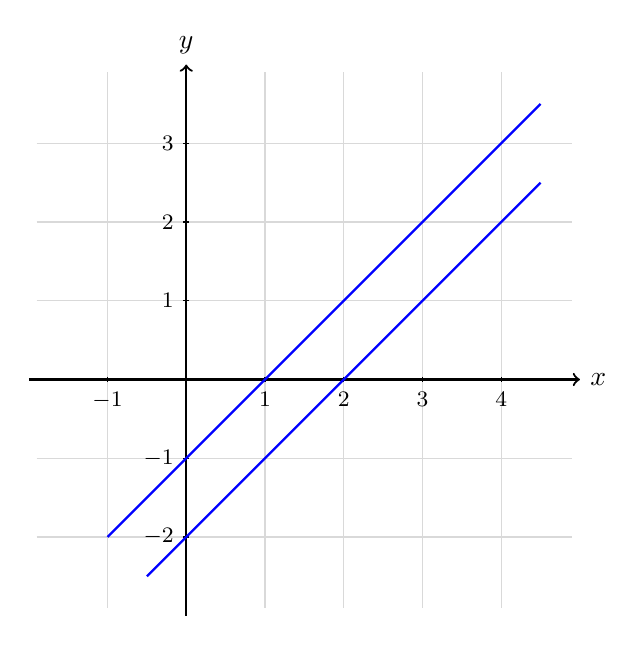
\begin{tikzpicture}[scale=1]
        % 1. Draw the grid (light gray)
        \draw[step=1.0,gray!30,thin] (-1.9,-2.9) grid (4.9,3.9);

        % 2. Draw the Axes
        \draw[->,thick] (-2,0) -- (5,0) node[right] {$x$};
        \draw[->,thick] (0,-3) -- (0,4) node[above] {$y$};

        % 3. Draw Ticks on Axes
        \foreach \x in {-1,1,2,3,4}
            \draw (\x,1pt) -- (\x,-1pt) node[below, font=\footnotesize] {$\x$};
        \foreach \y in {-2,-1,1,2,3}
            \draw (1pt,\y) -- (-1pt,\y) node[left, font=\footnotesize] {$\y$};

        % 4. Plot Line 1: y = x - 1 (Blue)
        % Since x - y = 1 implies y = x - 1
        \draw[blue, thick, domain=-1:4.5] plot (\x, {\x - 1});

        % 5. Plot Line 2: y = x - 2 (Red)
        % Since x - y = 2 implies y = x - 2
        \draw[blue, thick, domain=-0.5:4.5] plot (\x, {\x - 2});

    \end{tikzpicture}
    \item Jeśli są dwa różne zbiory $A, B \in \mathsf{P}(\mathbb{R})$, to BSO musi być takie $a$, że $a \in A$ oraz $a \notin B$. Wtedy $(0, a) \in F(A)$ i $(0, a) \notin F(B)$, czyli $F(A) = F(B)$. Zatem $F$ jest różnowartościowa. Zauważmy, że nie ma takiego $A$, że $F(A) = \{(0, 0)\}$, bo gdyby było, to musiałoby zachodzić $0 - 0 = 0 \in A$, czyli skoro $1-1 = 0 \in A$, to $(1, 1) \in F(A)$. Zatem $F$ nie jest surjekcją.
    \item Dla dowolnego $x$ zachodzi $x - x = 0 \in \N$, czyli $(x, x) \in F(\N)$, zatem relacja $F(\N)$ jest zwrotna. Jeśli $(x, y), (y, z) \in F(\N)$, to $y - x \in \N$ i $z - y \in \N$, czyli $(y - x) + (z - y) = z - x \in \N$, czyli $(x, z) \in F(\N)$, czyli relacja $F(\N)$ jest przechodnia. Jeśli $(x, y), (y, x) \in F(\N)$, to $x - y$ i $y - x$ są liczbami naturalnymi, czyli obie są nieujemne, czyli $x = y$, czyli relacja $F(\N)$ jest antysymetryczna. Zatem $F(\N)$ jest porządkiem częściowym.\\
    Przykładowym antyłańcuchem jest zbiór $\{n\sqrt2 : n \in \N\}$. Jeśli dwa elementy są z sobą w relacji, czyli dla pewnych różnych $n, m \in \N$ zachodzi $(n\sqrt2, m\sqrt2) \in F(\N)$, to $m\sqrt2 - n\sqrt2 = (m - n)\sqrt2 \in \N$, co jest sprzeczne z tym, że $\sqrt2$ jest niewymierne.
    \item Jeśli $A \in \mathsf{P}(\R)$ jest takie, że $F(A)$ jest relacją zwrotną, to $(0, 0) \in F(A)$, czyli $0 - 0 = 0 \in A$. Jeśli $0 \in A$, to dla dowolnego $x \in \R$ zachodzi $x - x = 0 \in A$, czyli $(x, x) \in F(A)$, czyli $F(A)$ jest zwrotna. Zatem przeciwobrazem zbioru relacji zwrotnych jest rodzina zbiorów zawierających 0.
    \item $F(\Q)$ zawiera $(x, x)$ dla dla dowolnego $x \in \R$, bo $x - x = 0 \in \Q$, zatem $|F(\Q)| \geq |\Q| = \aleph_0$. Wiemy też, że $F(\Q) \subseteq \Q^2$, więc $|F(\Q)| \leq |\Q^2| = \aleph_0$. Zatem $|F(\Q)| = \aleph_0$.
\end{enumerate}
\end{rozwiazanie}

\end{document}